\section{Langkah-Langkah Percobaan}
\begin{enumerate}
    \item Routing Statis IPv6
    \begin{enumerate}
        \item Masuk ke Winbox pada masing-masing router. Bila 
        router belum reset, maka lakukan reset terlebih dahulu.

        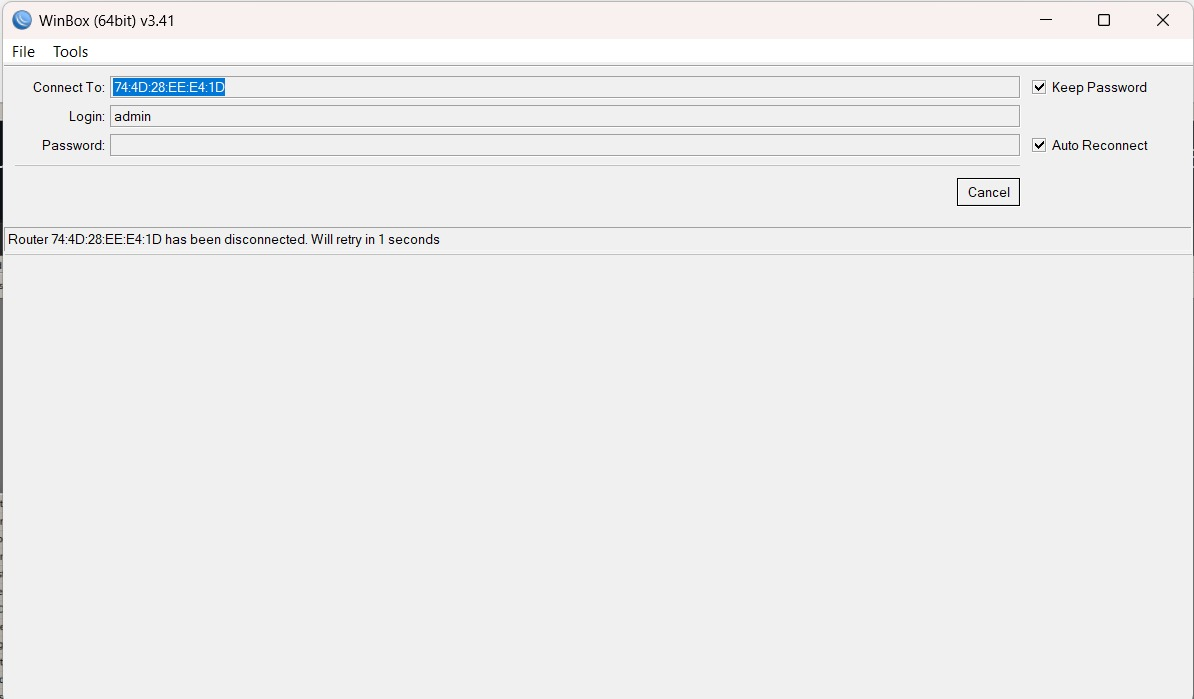
\includegraphics[scale=0.2]{P1/img/1.jpg}

        \item check Package List dan pastikan IPv6 sudah dijalankan.
        
        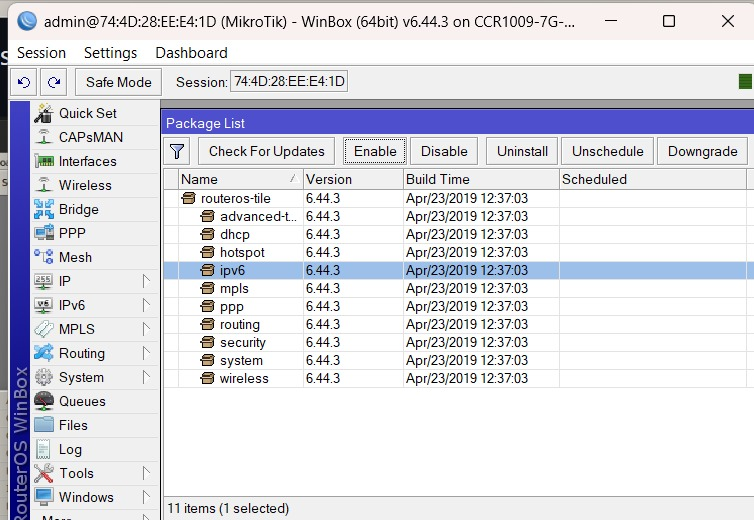
\includegraphics[scale=0.4]{P1/img/3.jpg}

        \item Konfigurasi IP Address pada Ether1 (note lakukan 
        konfigurasi ini pada router A dan B) Tambahkan IP 
        address pada ether1 yang digunakan sebagai jalur 
        antar-router. Karena hanya ada dua perangkat yang terhubung 
        (router A dan router B),

        \begin{itemize}
            \item IP ether1 Router A : 2001:db8:1::1/64
            \item IP ether 1 Router B : 2001:db8:1::2/64
        \end{itemize}

        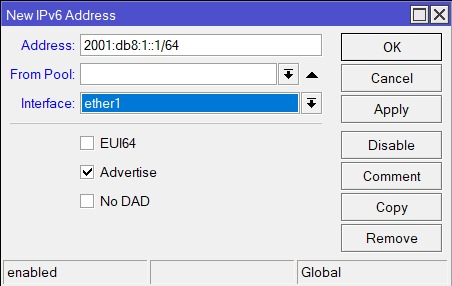
\includegraphics[scale=0.6]{P1/img/5.jpg}

        \item Konfigurasi IP Address untuk Jaringan LAN (note 
        lakukan konfigurasi ini pada router A dan b) Tambahkan 
        IP address pada ether 2 yang digunakan untuk 
        menghubungkan Laptop dengan Router.

        \begin{itemize}
            \item IP ether 2 Router A : 2001:db8:a::1/64
            \item IP ether 2 Router B : 2001:db8:b::1/64
        \end{itemize}

        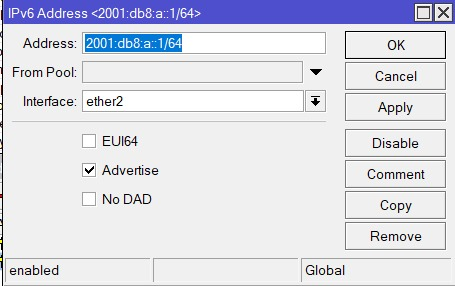
\includegraphics[scale=0.6]{P1/img/6.jpg} \newline
        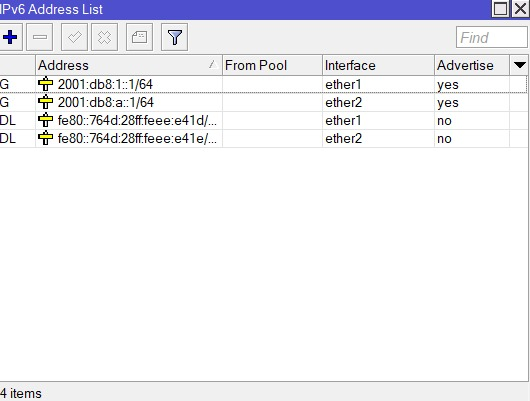
\includegraphics[scale=0.6]{P1/img/7.jpg}

        \item Konfigurasi Routing Statis (note lakukan 
        konfigurasi ini pada router A dan b) Setelah semua 
        interface diberi IP, langkah selanjutnya adalah menambahkan 
        rute secara manual. Masuk ke menu IPv6 → Routes, kemudian 
        klik "+" untuk menambahkan routing. Pada Router 1

        \begin{itemize}
            \item Dst. Address: 2001:db8:b::/64
            \item Gateway: 2001:db8:1::2
        \end{itemize}
        Pada Router 2
        \begin{itemize}
            \item Dst. Address: 2001:db8:a::/64
            \item Gateway: 2001:db8:1::1
        \end{itemize}

        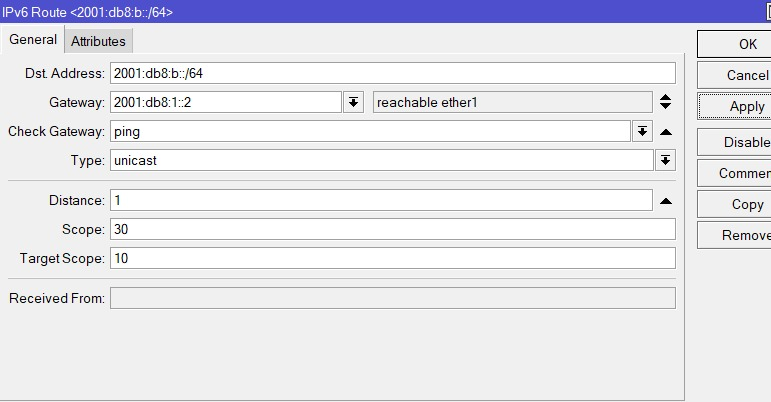
\includegraphics[scale=0.4]{P1/img/8.jpg}

        \item Kita dapat test ping router antara router untuk 
        memastikan routing statis antar router sudah berhasil.

        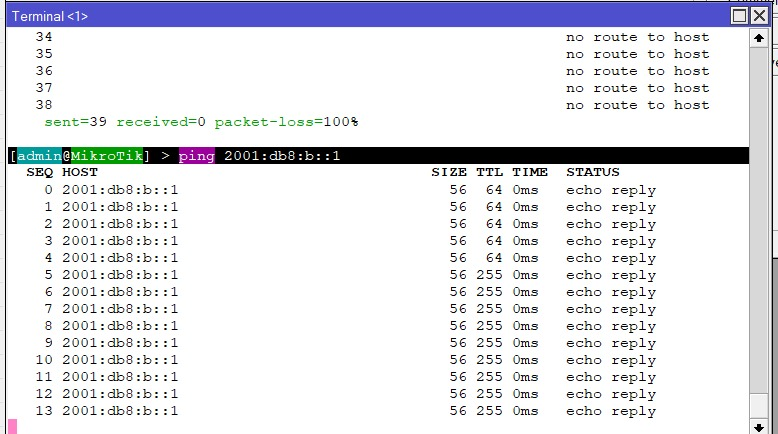
\includegraphics[scale=0.4]{P1/img/9.jpg}
        
        \item Konfigurasi IP Adress di Laptop (note lakukan 
        konfigurasi ini laptop yang terhubung pada router A dan 
        b masing-masing) Karena ini masih menggunakan konfigurasi 
        Static IP tambahkan IP address secara manual ke 
        interface di laptop masing-masing bisa lewat Control 
        Panel atau langsung di settings Windows, pastikan IP 
        dan Gateway sudah benar sesuai Ether 2. Pada laptop yang 
        terhubung ke Router 1
        \begin{itemize}
            \item IP Address: 2001:db8:a::100
            \item Prefix : /64
            \item Gateway : 2001:db8:a::1 (Router1)
            \item DNS :2001:4860:4860::8888
        \end{itemize}
        Pada laptop yang terhubung ke Router 2
        \begin{itemize}
            \item IP Address: 2001:db8:b::100
            \item Prefix : /64
            \item Gateway : 2001:db8:b::1 (Router2)
            \item DNS :2001:4860:4860::8888
        \end{itemize}

        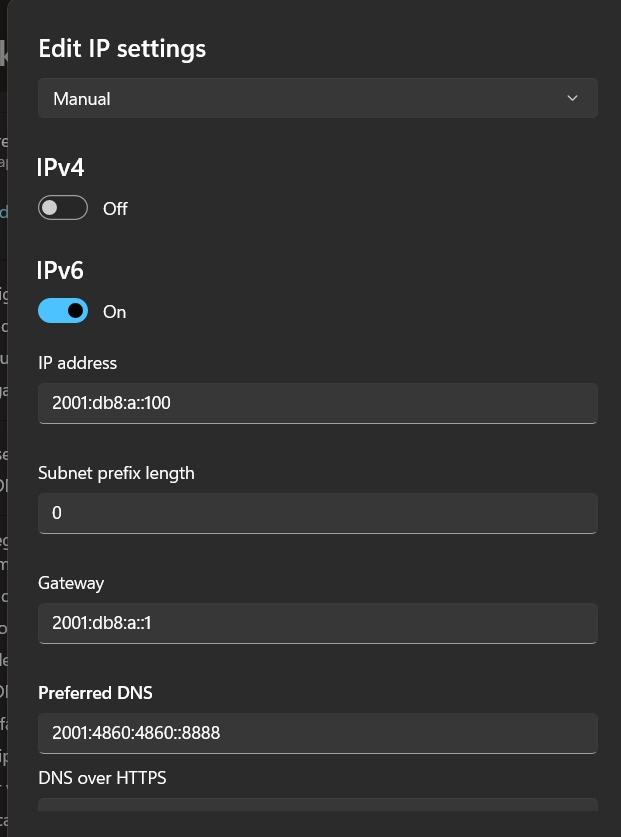
\includegraphics[scale=0.4]{P1/img/10.jpg} 

        \item Kita dapat melakukan ping antar laptop untuk 
        memastikan konfigurasi IP statis sudah berhasil.

        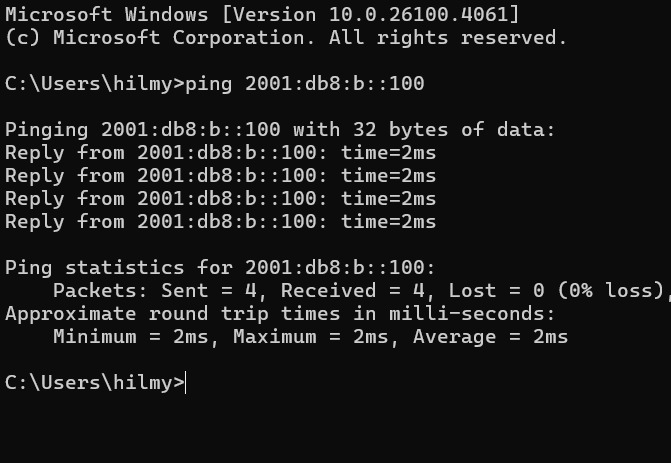
\includegraphics[scale=0.6]{P1/img/11.jpg}

    \end{enumerate}
    \item Routing Dinamis IPv6
    
    \begin{enumerate}
        \item Masuk ke Winbox pada masing-masing router. Bila 
        router belum reset, maka lakukan reset terlebih dahulu.

        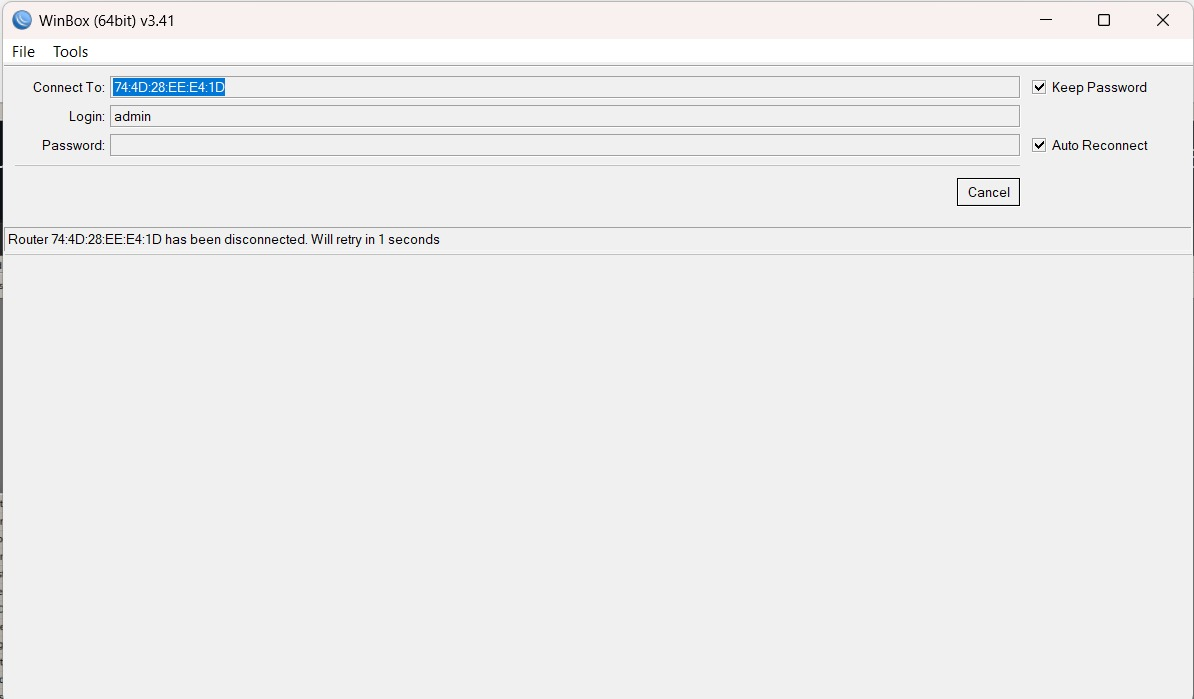
\includegraphics[scale=0.2]{P1/img/1.jpg}

        \item check Package List dan pastikan IPv6 sudah dijalankan.
        
        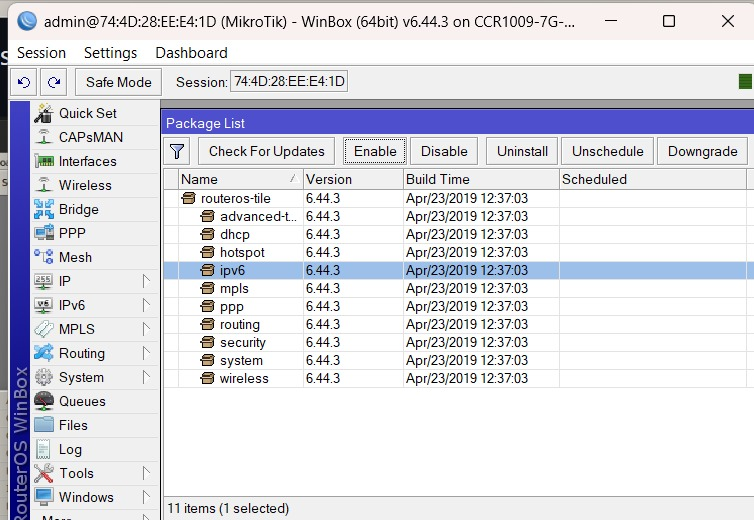
\includegraphics[scale=0.4]{P1/img/3.jpg}

        \item Konfigurasi IP Address pada Ether1 (note lakukan 
        konfigurasi ini pada router A dan B) Tambahkan IP 
        address pada ether1 yang digunakan sebagai jalur 
        antar-router. Karena hanya ada dua perangkat yang terhubung 
        (router A dan router B),

        \begin{itemize}
            \item IP ether1 Router A : 2001:db8:1::1/64
            \item IP ether 1 Router B : 2001:db8:1::2/64
        \end{itemize}

        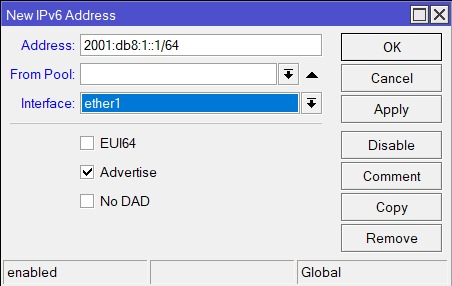
\includegraphics[scale=0.6]{P1/img/5.jpg}

        \item Konfigurasi IP Address untuk Jaringan LAN (note 
        lakukan konfigurasi ini pada router A dan b) Tambahkan 
        IP address pada ether 2 yang digunakan untuk 
        menghubungkan Laptop dengan Router.

        \begin{itemize}
            \item IP ether 2 Router A : 2001:db8:a::1/64
            \item IP ether 2 Router B : 2001:db8:b::1/64
        \end{itemize}

        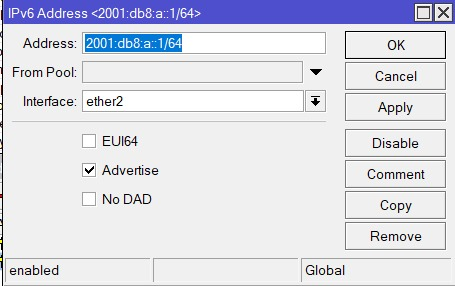
\includegraphics[scale=0.6]{P1/img/6.jpg} \newline
        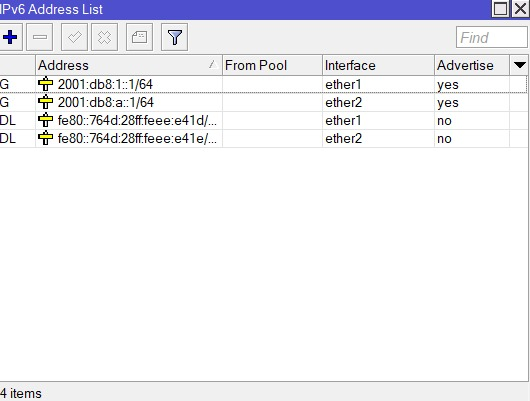
\includegraphics[scale=0.6]{P1/img/7.jpg}

        \item Masuk ke menu OSPFv3 dan buat instansi baru.
        
        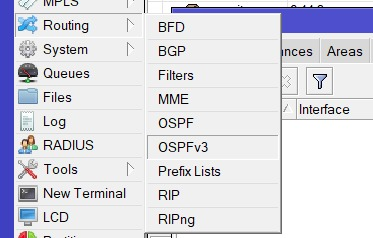
\includegraphics[scale=0.6]{P1/img/12.jpg}

        \item Buat instansi OSPFv3 seperti berikut:
        \begin{itemize}
            \item Masuk ke menu IIPv6 > Routing > OSPFv3 > Instances → Klik + untuk menambahkan routing.
            \item Name: ospf-instance
            \item Router ID: misalnya 1.1.1.1 untuk Router1, 2.2.2.2 untuk Router2
        \end{itemize}
        
        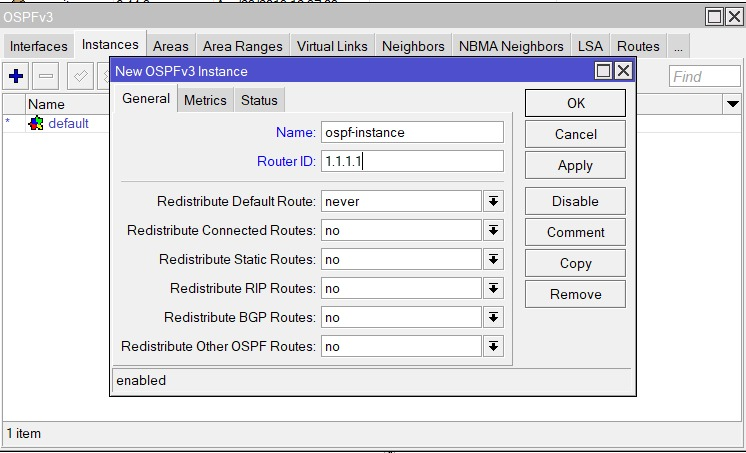
\includegraphics[scale=0.5]{P1/img/13.jpg}

        \item Tambah area OSPFv3 seperti berikut:
        \begin{itemize}
            \item Masuk ke menu Routing > OSPFv3 > Areas → Klik +
            \item Name: backbone
            \item Instance: pilih ospf-instance
            \item Area ID: 0.0.0.0 (wajib untuk backbone area)
        \end{itemize}

        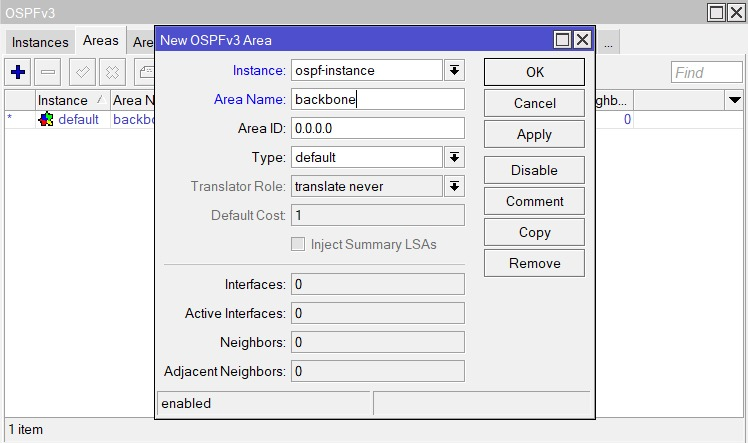
\includegraphics[scale=0.5]{P1/img/14.jpg}

        \item Tambah interface OSPFv3 seperti berikut:
        \begin{itemize}
            \item Router1:
            \item Masuk ke menu Routing > OSPFv3 > Interface → Klik +
            \item Interface: ether1 (ke Router2)
            \item Instance: ospf-instance
            \item Area: backbone Tambahkan juga interface LAN:
            \item Interface: ether2 Router2:
            \item Tambahkan interface ether1 dan ether2 dengan cara yang sama
        \end{itemize}

        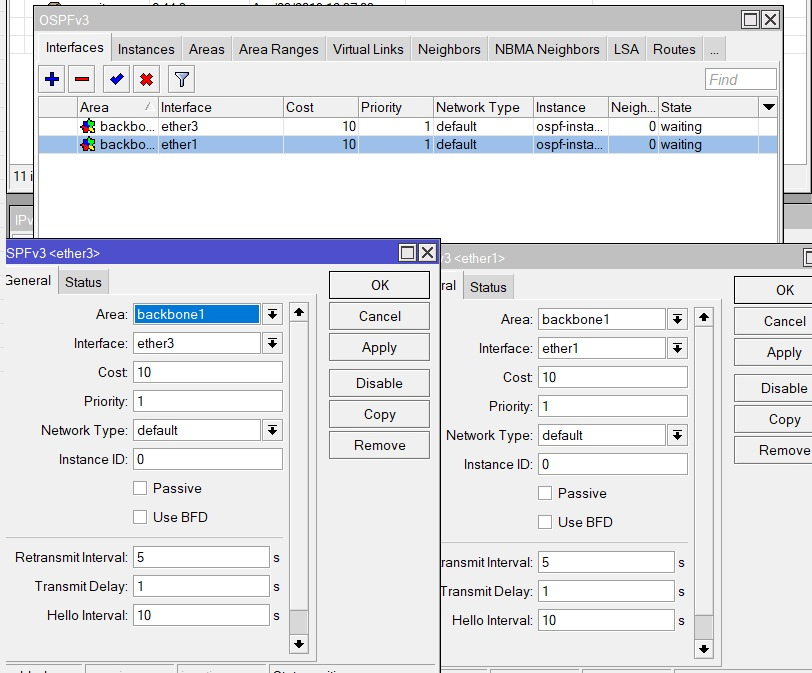
\includegraphics[scale=0.5]{P1/img/15.jpg}

        \item Cek Neighbor dan Routing Masuk ke menu Routing > OSPFv3 > Neighbors
        \begin{itemize}
            \item Harus muncul tetangga OSPF antara Router1 dan Router2 Optional coba cek Masuk ke menu IPv6 > Routes
            \item Harus terlihat rute dinamis ke jaringan 2001:db8:a::/64 dan 2001:db8:b::/64
        \end{itemize}

        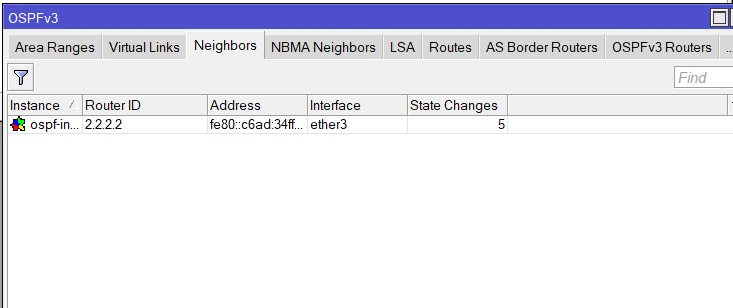
\includegraphics[scale=0.5]{P1/img/16.jpg}

        \item Konfigurasi IP Adress di Laptop (note lakukan 
        konfigurasi ini laptop yang terhubung pada router A dan 
        b masing-masing) Karena ini masih menggunakan konfigurasi 
        Static IP tambahkan IP address secara manual ke 
        interface di laptop masing-masing bisa lewat Control 
        Panel atau langsung di settings Windows, pastikan IP 
        dan Gateway sudah benar sesuai Ether 2. Pada laptop yang 
        terhubung ke Router 1
        \begin{itemize}
            \item IP Address: 2001:db8:a::100
            \item Prefix : /64
            \item Gateway : 2001:db8:a::1 (Router1)
            \item DNS :2001:4860:4860::8888
        \end{itemize}
        Pada laptop yang terhubung ke Router 2
        \begin{itemize}
            \item IP Address: 2001:db8:b::100
            \item Prefix : /64
            \item Gateway : 2001:db8:b::1 (Router2)
            \item DNS :2001:4860:4860::8888
        \end{itemize}

        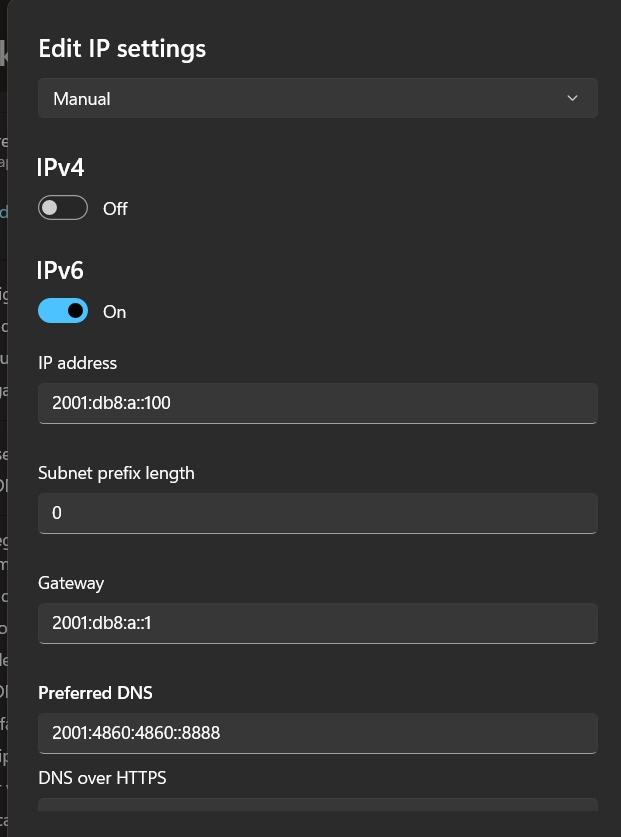
\includegraphics[scale=0.4]{P1/img/10.jpg} 

        \item Jika Sudah Uji test PING dari Laptop 1 ke alamat Laptop 2, Jika berhasil maka Routing tidak ada masalah.
        
        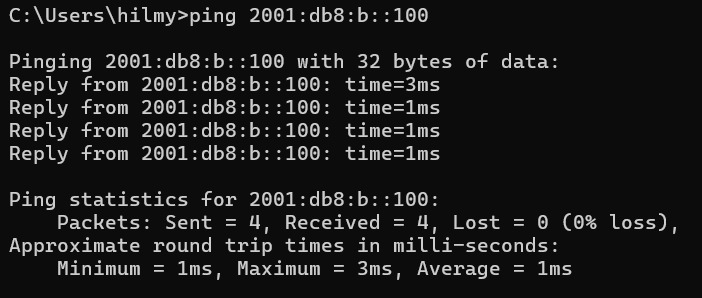
\includegraphics[scale=0.6]{P1/img/17.jpg}

    \end{enumerate}
\end{enumerate}
\section{Analisis Hasil Percobaan}
\begin{enumerate}
    \item Routing Statis IPv6
    
    Dalam percobaan ini, dua router MikroTik dihubungkan dan 
    dikonfigurasikan untuk berkomunikasi melintasi subnet yang 
    berbeda menggunakan rute statis yang ditentukan secara manual. 
    Setiap router menerima alamat IPv6 pada antarmuka yang 
    digunakan untuk menghubungkan ke router lain, dan rute 
    statis ditambahkan untuk memungkinkan komunikasi antara 
    jaringan masing-masing. Manfaat utama dari perutean statis 
    terletak pada kesederhanaannya dan kontrol yang tepat yang 
    ditawarkannya - administrator jaringan dapat menentukan 
    jalur yang tepat untuk lalu lintas, membuat manajemen 
    menjadi mudah dan dapat diprediksi. Namun, perutean statis 
    tidak beradaptasi dengan perubahan dalam jaringan secara 
    otomatis. Jika sebuah router mati atau topologi berubah, 
    rute harus diperbarui secara manual. Karena itu, perutean 
    statis umumnya lebih cocok untuk jaringan yang lebih kecil 
    dan stabil-seperti yang ada di rumah atau lingkungan kantor 
    kecil-di mana fleksibilitas tidak terlalu penting 
    dibandingkan dengan stabilitas dan kontrol.

    \item Routing Dinamis IPv6
    
    Percobaan perutean dinamis menggunakan OSPFv3 untuk 
    memungkinkan dua router MikroTik untuk berbagi informasi 
    perutean secara otomatis. Hal ini memungkinkan setiap router 
    untuk menentukan jalur terbaik yang tersedia ke tujuan tanpa 
    konfigurasi rute manual. Keuntungan utama dari penggunaan 
    OSPFv3 adalah daya tanggapnya terhadap perubahan di dalam 
    jaringan. Jika sebuah router gagal atau sebuah sambungan 
    tidak tersedia, OSPFv3 akan dengan cepat menemukan dan 
    beralih ke jalur alternatif, memastikan komunikasi terus 
    berlanjut. Hal ini membuatnya sangat efektif dalam jaringan 
    yang lebih besar atau yang terus berubah. Perutean dinamis 
    juga menyederhanakan manajemen dengan mendistribusikan 
    informasi rute secara otomatis. Namun, hal ini memiliki 
    kekurangan - OSPFv3 lebih rumit untuk diatur dan 
    mengkonsumsi lebih banyak sumber daya sistem dibandingkan 
    dengan perutean statis.
\end{enumerate}
\section{Hasil Tugas Modul}
\begin{enumerate}
    \item Simulasikan Konfigurasi Praktikum P2 di atas mengenai Routing Dinamis dan Statis IPV6 menggunakan GNS3

    Berikut adalah topologi yang digunakan untuk menjalankan 
    simulasi routing statis dan dinamis IPv6 pada Cisco Packet 
    Tracer karen teman-teman saya tidak menggunakan GNS3.

    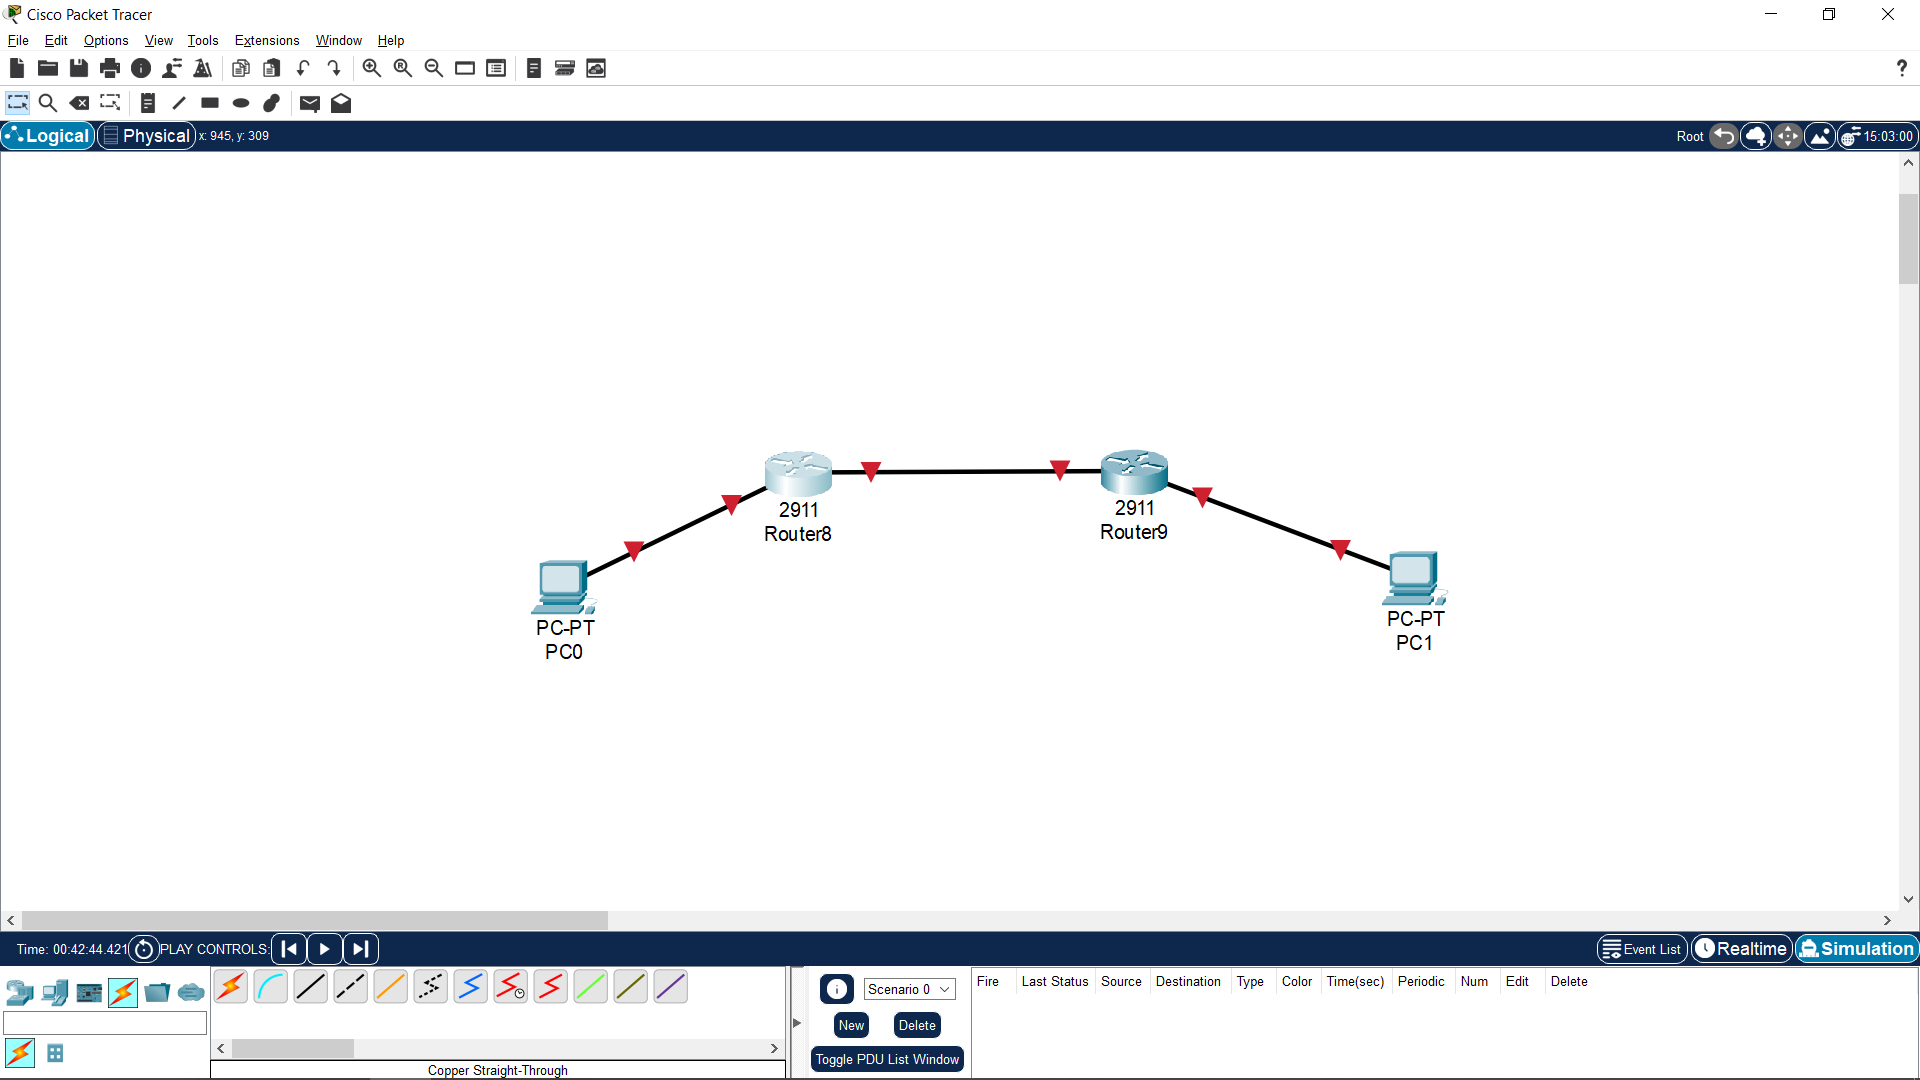
\includegraphics[scale=0.17]{P1/img/19.png}
\end{enumerate}
\section{Kesimpulan}
Perutean Statis IPv6 paling cocok untuk jaringan berskala kecil 
atau yang relatif stabil di mana perubahan jarang terjadi. 
Keuntungan utamanya adalah tingkat kontrol yang 
disediakannya-setiap rute ditentukan secara manual, yang 
memungkinkan administrator jaringan mengelola jalur lalu lintas 
dengan presisi. Kesederhanaan ini membuat perutean statis mudah 
dikonfigurasi dan dipecahkan masalahnya, dan biasanya 
menggunakan lebih sedikit sumber daya sistem dibandingkan dengan 
protokol dinamis. Namun, pendekatan ini memiliki keterbatasan 
yang signifikan dalam lingkungan yang lebih dinamis. Rute statis 
tidak menyesuaikan secara otomatis terhadap perubahan topologi 
jaringan, seperti router yang gagal atau perangkat yang baru 
ditambahkan. Dalam kasus seperti itu, rute harus diperbarui 
secara manual, yang dapat memakan waktu dan rentan terhadap 
kesalahan seiring pertumbuhan jaringan. Oleh karena itu, 
meskipun perutean statis menawarkan stabilitas dan kontrol, 
umumnya paling efektif dalam jaringan kecil di mana perubahan 
rute jarang terjadi.

Perutean Dinamis IPv6, seperti dengan OSPFv3, dirancang untuk 
jaringan yang lebih besar dan lebih kompleks di mana kemampuan 
beradaptasi dan skalabilitas adalah kuncinya. Protokol perutean 
dinamis secara otomatis bertukar informasi perutean antara 
router, memungkinkan mereka untuk menentukan jalur optimal 
secara real time. Ini berarti bahwa jika router atau koneksi 
terputus, jaringan dapat dengan cepat mengalihkan lalu lintas 
tanpa intervensi manual. Kemampuan beradaptasi ini meningkatkan 
keandalan dan meminimalkan waktu henti, terutama di jaringan 
yang sering mengalami perubahan atau perluasan konfigurasi. 
Perutean dinamis juga mengurangi beban administratif untuk 
memelihara tabel rute secara manual. Namun, peningkatan 
kompleksitas pengaturan dan penggunaan sumber daya yang lebih 
tinggi dapat dilihat sebagai kelemahan, terutama di lingkungan 
yang lebih kecil di mana kemampuan beradaptasi seperti itu tidak 
diperlukan. Meskipun demikian, untuk jaringan yang sedang 
berkembang atau lingkungan perusahaan, perutean dinamis 
menawarkan fleksibilitas dan ketahanan yang diperlukan untuk 
menjaga komunikasi yang efisien dan berkelanjutan.
\section{Lampiran}
\subsection{Dokumentasi saat praktikum}
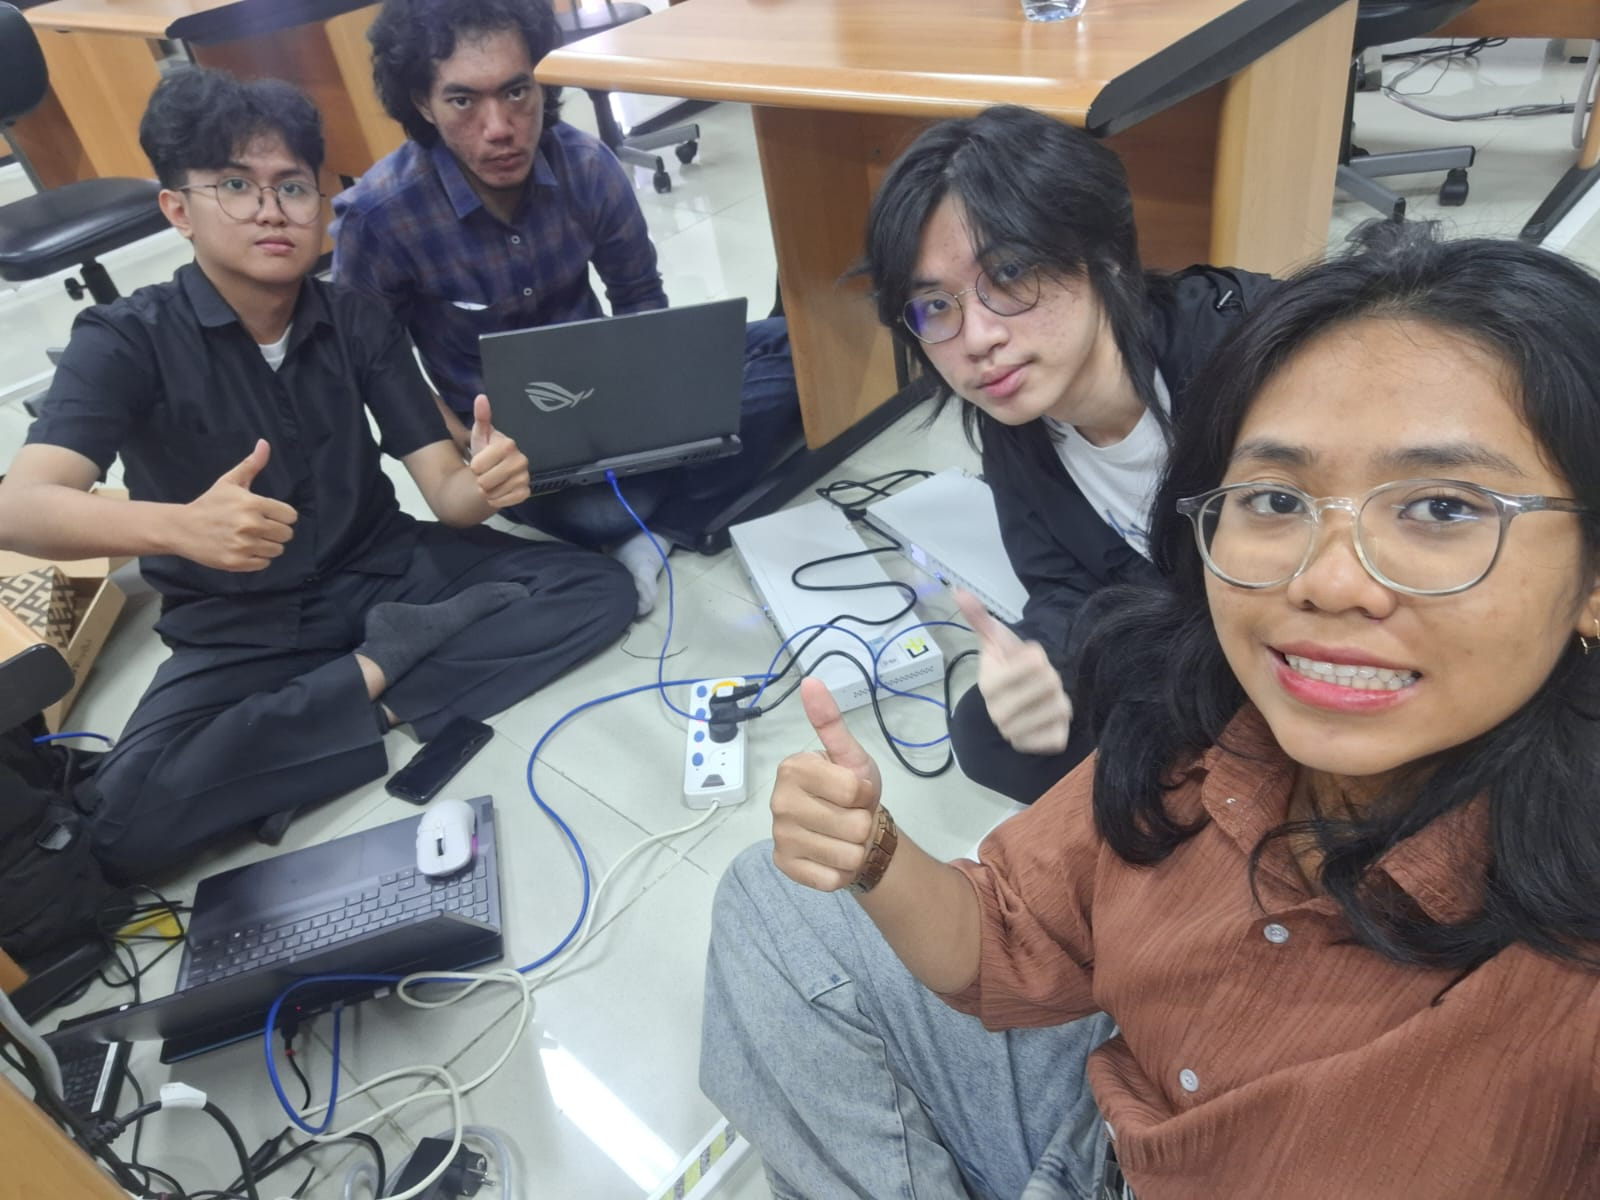
\includegraphics[scale=0.3]{P1/img/18.jpg}